\documentclass[a4paper, 11pt]{article}


\usepackage[utf8]{inputenc}
\usepackage[frenchb]{babel}
\usepackage[T1]{fontenc}
\usepackage{textcomp}
\usepackage{amsmath,amssymb}
\usepackage{lmodern}
\usepackage[a4paper]{geometry}
\usepackage{graphicx}
\usepackage{xcolor}
\usepackage{microtype}
\usepackage{listings}
\usepackage{hyperref}
\usepackage{float}
\usepackage{listings}
\usepackage{color}
\definecolor{dkgreen}{rgb}{0,0.6,0}
\definecolor{gray}{rgb}{0.5,0.5,0.5}
\definecolor{mauve}{rgb}{0.58,0,0.82}
\DeclareUnicodeCharacter{00A0}{ }
\lstset{frame=tb,
  language=Matlab,
  aboveskip=3mm,
  belowskip=3mm,
  showstringspaces=false,
  columns=flexible,
  basicstyle={\small\ttfamily},
  numbers=none,
  numberstyle=\tiny\color{gray},
  keywordstyle=\color{blue},
  commentstyle=\color{dkgreen},
  stringstyle=\color{mauve},
  breaklines=true,
  breakatwhitespace=true,
  tabsize=3
}

\renewcommand*{\familydefault}{\sfdefault}


\title{Rapport D'Analyse : Aide à la Décision}


\author{Yassine Moreno \cr Mehdi Kitane \cr Amine ElRhazi \cr Abdelalim Tribak \cr Meryem Benchakroune \cr Karim Benhmida}

\begin{document}

\begin{LARGE}
\maketitle
\end{LARGE}

\tableofcontents
\newpage

\section{Introduction}
\subsection{Mise en situation}
L'objectif de ce document est de présenter la démarche ainsi que le modèle mathématique choisi pour établir le meilleur plan de production pour l'entreprise $FaBrique$. Cette solution prendra en compte toutes les contraintes spécifiées par les différents acteurs au sein de l'entreprise. 
\subsection{Concepts généraux et Contraintes}
\subsection*{Concepts généraux}
On considèrera dans tout ce qui suit : \\
- $X = \begin{pmatrix}
        a\\
        b\\
        c\\
        d\\
        e\\
        f\\
    \end{pmatrix}$ le vecteur définissant la quantité hebdomadaire à fabriquer pour chaque produit (\textbf{variables de décision}).\\
- $Mchn = \left\{1, 2, 3, 4, 5, 6, 7\right\}$ l'ensemble des machines utilisées dans la fabrication des produits.\\
- $Mtr = \left\{MP1,MP2,MP3\right\}$ l'ensemble des matières premières utilisées lors de la confection des produits.
\subsection*{Jeu de contraintes}
Nous détaillerons dans cette section les contraintes imposées par les différents constituants de l'entreprise FaBrique. \\
Tout d'abord, les contraintes de domaine stipulent que toutes les quantités hebdomadaires à fabriquer par l'entreprise doivent être positifs ou nuls, ce qui peut se traduire par l'inégalité suivante :
\begin{center}
$$0 \leq X \Leftrightarrow 0 \leq a ,0 \leq b ,0 \leq c ,0 \leq d ,0 \leq e ,0 \leq f $$
\end{center}
Ensuite, les contraintes imposées par la quantité maximale de matières premières admissible : \textbf{350 unités pour MP1, 620 unités pour MP2 et 485 unités pour MP3}. Ces contraintes se traduiront par les inégalités suivantes :
$$
\left\{\begin{split}
	a+2b+c+5d+2f \leq 350 \\
    2a+2b+c+2d+2e+f  \leq 620 \\
    a+3c+2d+2e \leq 485 \\
\end{split}\right. \Leftrightarrow \begin{pmatrix}
        1&2&1&5&0&2 \\
        2&2&1&2&2&1\\
        1&0&3&2&2&0\\
    \end{pmatrix} \cdot X \leq \begin{pmatrix}
        350 \\
        620\\
        485\\
    \end{pmatrix}
$$
Enfin, les contraintes traduisant le volume horaire \textbf{hebdomadaire} maximal du fonctionnement des machines, ne dépassant pas 16 heures par jour, 5 jours par semaine -un total de \textbf{4800 minutes} hebdomadaires-.
$$
\left\{\begin{split}
	8a+15b+5d+10f \leq 4800 \\
    7a+b+2c+15d+7e+12f \leq 4800 \\
    8a+b+11c+10e+25f \leq 4800 \\
    2a+10b+5c+4d+13e+7f \leq 4800 \\
    5a+7d+10e+25f \leq 4800 \\
	5a+3b+5c+8d+7f \leq 4800\\
	5a+5b+3c+12d+8e \leq 4800\\
\end{split}\right. \Leftrightarrow \begin{pmatrix}
        8&15&0&5&0&10 \\
        7&1&2&15&7&12\\
        8&1&11&0&10&25\\
        2&10&5&4&13&7\\
        5&0&0&7&10&25\\
        5&3&5&8&0&7\\
        5&5&3&12&8&0
    \end{pmatrix} \cdot X \leq \begin{pmatrix}
        4800\\
        4800\\
        4800\\
        4800\\
        4800\\
        4800\\
        4800
    \end{pmatrix}
$$ \\
La matrice de contraintes complète\footnote{Matrice A} est disponible en \textbf{Annexe}.
\section{Programmation Linéaire Monocritère}
\subsection{Modélisation et Proposition de solution : Comptable}
L'objectif du comptable est de maximiser le bénéfice, ce dernier est obtenu par la différence entre le revenu global $G$ et des charges totales $C$  liées à l'achat des matières premières et du cout d'usinage sur les machines de l'entreprise.\\
Ainsi la fonction objectif du problème de comptabilité se modélise sous la forme suivante :
\begin{center}
$F_{compta} (X) = G(X) - C(X)$ \\
\end{center}
En considérant les fonctions suivantes : \\
- Le revenu global :\\
$G(X) = (20~27~26~30~45~40)\cdot X $ \\
$G(X) =  20\cdot a + 27\cdot b + 26\cdot c + 30\cdot d + 45\cdot e + 40\cdot f $ \\
- Les charges totales :\\
$C(X) = C_{mtrprem}(X) + C_{machines}(X) $ \\ 
Pour les matières premières :
$C_{mtrprem}(X) = \sum_{i\in{X}}{Cmtp_i\cdot i} $ \\
$Prix = \begin{pmatrix}
        3\\
        4\\
        2\\
    \end{pmatrix}$
$$
\begin{array}{r l}
    Cmtp_a = & (1~2~1)\cdot Prix = 13 \\
    Cmtp_b = & (2~2~0)\cdot Prix = 14 \\
    Cmtp_c = & (1~1~3)\cdot Prix = 15 \\
    Cmtp_d = & (5~2~2)\cdot Prix = 27 \\
    Cmtp_e = & (0~2~2)\cdot Prix = 12 \\
    Cmtp_f = & (2~1~0)\cdot Prix = 10 \\
\end{array}
$$
\\
D'où : $C_{mtrprem}(X) = 13\cdot a + 14\cdot b + 15\cdot c + 27\cdot d + 12\cdot e + 10\cdot f  $ \\
Pour les couts d'usinage :\\
$C_{machines}(X) = \sum_{i\in{X}}{Cmachines_i\cdot i} $ \\

$CoutMinute = \begin{pmatrix}
        0.03\\
        0.03\\
        0.017\\
        0.017\\
        0.03\\
        0.05\\
        0.05\\
    \end{pmatrix}$
$$
\begin{array}{r r l l}
    Cmachines_a = & (8~7~8~2~5~5~5)\cdot  & CoutMinute = & 1.33 \\
    Cmachines_b = & (15~1~1~10~0~5~3)\cdot   & CoutMinute = & 1.11 \\
    Cmachines_c = & (0~2~11~5~0~3~5)\cdot   & CoutMinute = & 0.73 \\
    Cmachines_d = & (5~15~0~4~7~12~8)\cdot   & CoutMinute = & 1.96 \\
    Cmachines_e = & (0~7~10~13~10~8~0)\cdot  & CoutMinute = & 1.35 \\
    Cmachines_f = & (10~12~25~7~25~0~7)\cdot & CoutMinute = & 2.45 \\
\end{array}
$$
D'où : $C_{machines}(X) = 1.33\cdot a + 1.11\cdot b + 0.73\cdot c + 1.96\cdot d + 1.35\cdot e + 2.45\cdot f  $ \\
Ainsi, nous pouvons déduire la fonction objectif -traduisant le bénéfice- à maximiser :
\begin{center}
$F_{compta} (X) = (5.67~11.88~12.27~1.03~31.65~27.55)\cdot X$ \\
\end{center}

De ce fait, nous avons effectué cette démarche en minimisant la fonction suivante tout en intégrant les contraintes spécifiés précédemment :
\begin{center}
$f(X) = -F_{compta} (X) = (-5.67~-11.88~-12.27~-1.03~-31.65~-27.55)\cdot X$ \\
\end{center}
$$
avec \left\{\begin{split}
	f(X)\ à\ minimiser\\
    A\cdot X \leq b\\
    0 \leq X
\end{split}\right.
$$
La solution proposée est la suivante :
$ X =\begin{pmatrix}
0\\
20.41\\
0\\
0\\
242.50\\
94.18
\end{pmatrix} $\\
Le bénéfice maximal envisageable est de : \textbf{10 512 €}
\subsection{Modélisation et Proposition de solution : Resp.Atelier}
L'objectif du responsable d'atelier est de maximiser la fabrication des produits. Autrement dit, maximiser la quantité totale des produits. 
Nous modéliserons la fonction objectif sous la forme suivante :
\begin{center}
$F_{respAtelier} (X) =(1~1~1~1~1~1)\cdot X$ \\
\end{center}
Ainsi, le problème est réduit à une fonction $f$ à minimiser tout en tenant compte des contraintes globales précédentes :
$f(X) = -F_{respAtelier} (X) =(-1~-1~-1~-1~-1~-1)\cdot X$ \\
$$
avec \left\{\begin{split}
	f(X)\ à\ minimiser\\
    A\cdot X \leq b\\
    0 \leq X
\end{split}\right.
$$

La solution proposée est la suivante :
$ X =\begin{pmatrix}
0\\
56.73\\
38.69\\
0\\
184.46\\
98.92
\end{pmatrix} $\\
La production maximale envisageable est de : \textbf{378.8 Produits}
\subsection{Modélisation et Proposition de solution : Resp.Stock}
La problématique du responsable des stocks est double, puisqu'il s'agit de minimiser le stock global de l'entreprise tout en préservant un niveau minimal d'activité au sein de l'entreprise.\\
Nous nous attaquerons dans un premier temps à la fonction objectif , obtenu par la somme des quantités des produits et des quantités de matières premières pour chaque produit :
\begin{center}
$F_{respStock} (X) =(1~1~1~1~1~1)+(4~4~5~9~4~3)\cdot X$ \\
$F_{respStock} (X) =(5~5~6~10~5~4)\cdot X$\\
\end{center}
Néanmoins, cette fonction -à minimiser- admet le vecteur nul comme solution minimale, réduisant à néant la productivité de l'entreprise.\\
De ce fait, afin de contourner le problème, nous ajouterons 2 contraintes supplémentaires concernant la production totale de l'entreprise pour traduire l'activité.\\
- La première contrainte, qui concerne la production maximale, se traduit par l'inégalité suivante :\\
\textbf{a+b+c+d+e+f < 378.8}\\
- La deuxième contrainte concerne un seuil minimal d'activité qui ne pourrait être inférieur à 50\% du maximum afin de maintenir un bénéfice acceptable pour l'entreprise :\\
\textbf{ 378.8*i < a+b+c+d+e+f avec 0.50<i<1}\\
\\
En intégrant les nouvelles contraintes au jeu établi précédemment par le biais de \textbf{$A_{new}$} et de \textbf{$b_{new}$} , nous avons pu modéliser l'évolution du stock global $F_{respStock} (X)$ en fonction du pourcentage $\%prodMax$ de la production maximale imposé en seuil minimal d'activité (cf. Figure 1).\\
\begin{figure}[H]
    \begin{center}
        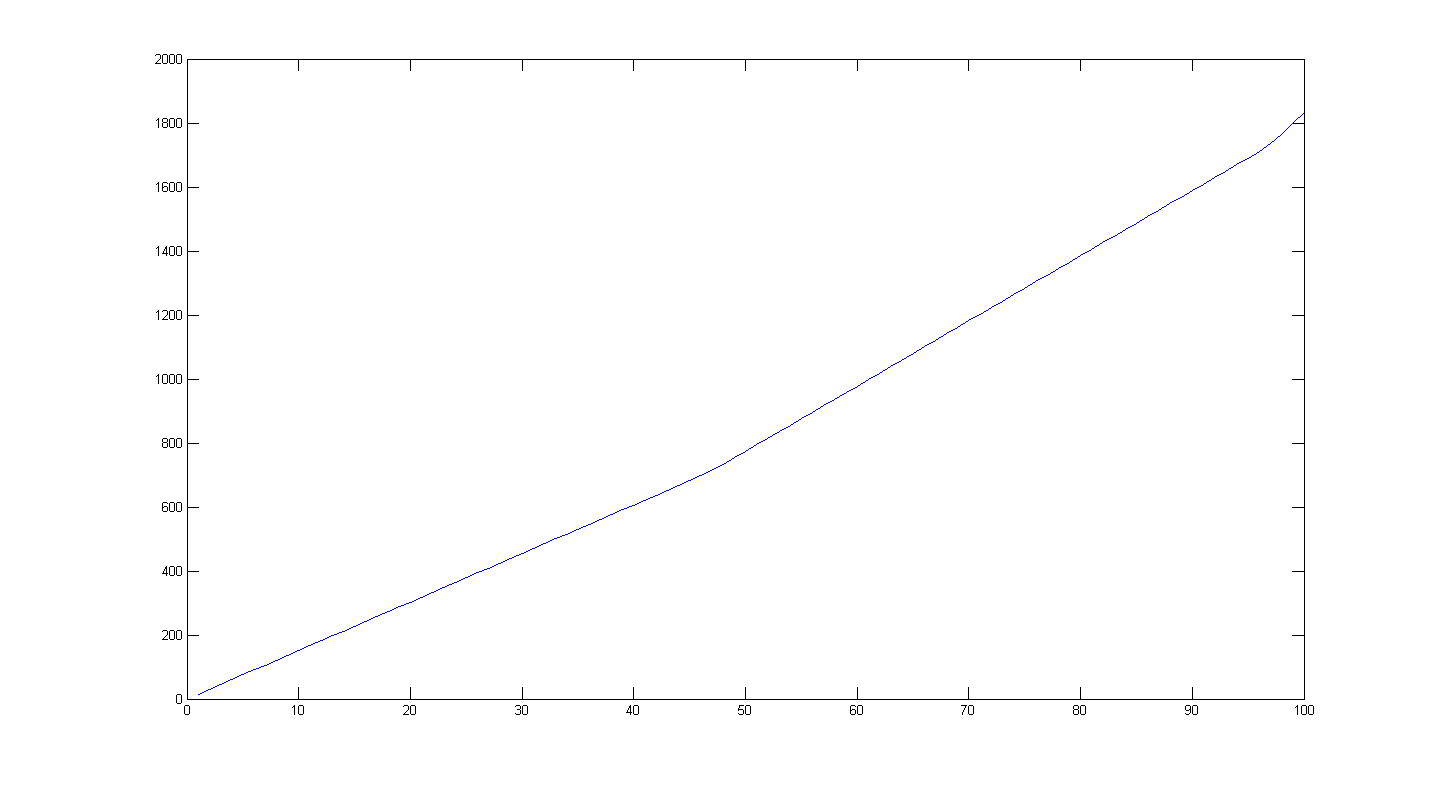
\includegraphics[scale=0.35]{Stock}
        \caption{
            \label{fig} Évolution du stock en fonction de \%prodMax
        }
    \end{center}
\end{figure}
Ainsi, nous constatons un point d'inflexion établi à \textbf{80\%} de la production maximale. Au delà, on constate une augmentation très rapide du stock qui ne satisfait nullement l'objectif fixé.
C'est à partir de ce point particulier que nous construirons notre solution au problème suivant :
$f(X) = F_{respStock} (X) =(5~5~6~10~5~4)\cdot X$ \\
$$
avec \left\{\begin{split}
	f(X)\ à\ minimiser\\
    A_{new}\cdot X \leq b_{new}\\
    0 \leq X
\end{split}\right.
$$
La solution optimale pour ce problème est la suivante :
$ X =\begin{pmatrix}
38.35\\
25.47\\
0\\
0\\
108.87\\
130.36
\end{pmatrix} $\\
Le stock minimal obtenu par ces données est de : \textbf{1384 unités}

\subsection{Modélisation et Proposition de solution : Resp.Commercial}
Le responsable commercial a pour objectif la réalisation de l'équilibre entre la première famille de produits (A,B et C) et la seconde (D,E et F). Cette contrainte d'égalité se modélise par l'équation suivante :
\begin{center}
$ a+ b+ c = d+ e+ f\Leftrightarrow(1~1~1~-1~-1~-1)\cdot X = 0 \Leftrightarrow A_{eq}\cdot X = b_{eq} $
\end{center}
Le fonction objectif du responsable commercial demeure identique à celle du responsable d'atelier, maximiser la production de l'entreprise -pour assurer l'activité de l'entreprise- tout en tenant compte de la nouvelle contrainte d'équilibre.
\begin{center}
$F_{respComm} (X) =(1~1~1~1~1~1)\cdot X$ \\
\end{center}
Ainsi, le problème est mathématiquement réduit à une fonction $f$ à minimiser tout en tenant compte des contraintes globales précédentes en plus de la nouvelle contrainte d'équilibre :
$f(X) = -F_{respComm} (X) =(-1~-1~-1~-1~-1~-1)\cdot X$ \\
$$
avec \left\{\begin{split}
	f(X)\ à\ minimiser\\
    A\cdot X \leq b\\
    A_{eq}\cdot X = b_{eq}\\
    0 \leq X
\end{split}\right.
$$
La solution optimale pour ce problème est la suivante :
$ X =\begin{pmatrix}
142.11\\
0\\
44.42\\
0\\
104.80\\
81.73
\end{pmatrix} $\\
La production de la première famille s'élève à \textbf{186.53 unités}\\
La production de la deuxième famille s'élève à \textbf{186.53 unités}\\
L'écart théorique constaté entre ces deux familles est de : \textbf{0 unités}
\subsection{Modélisation et Proposition de solution : Resp.Personnel}
La problématique du responsable du personnel concerne la réduction de l'usage des machines 3 et 5 tout en maintenant une activité correcte de l'entreprise.
La fonction objectif modélisant le problème se retranscrit sous la forme suivante :
\begin{center}
$F_{respPers} (X) =F_{TmpsMachine3} (X) + F_{TmpsMachine5} (X)$\\
$F_{TmpsMachine3} (X) = (8~1~11~0~10~25)\cdot X$\\
$F_{TmpsMachine5} (X) = (5~0~0~7~10~25)\cdot X$\\
$F_{respPers} (X) =(13~1~11~7~20~50)\cdot X$
\end{center}

Cependant, le minimum envisageable pour cette fonction est le vecteur nul, solution absurde pour assurer l'activité de l'entreprise. Ainsi, de manière identique au problème du responsable des stocks, nous ajouterons 2 contraintes supplémentaires liées à l'activité maximale de l'entreprise.
- La première contrainte, qui concerne la production maximale, se traduit par l'inégalité suivante :
\textbf{a+b+c+d+e+f < 378.8}\\
- La deuxième contrainte concerne un seuil minimal (pourcentage de la production maximale, à définir) d'activité :
\textbf{ 378.8*i < a+b+c+d+e+f avec 0<i<1}\\
A partir du jeu de contraintes modifié interprété par \textbf{$A_{new}$} et de \textbf{$b_{new}$}, nous pouvons établir une relation traduisant l'impact du seuil minimal sur les temps d'usinage des machines 3 et 5 ainsi que sur le temps d'utilisation global (cf. Figure 2)\\
\begin{figure}[H]
    \begin{center}
        \includegraphics[scale=0.38]{Pers}
        \caption{
            \label{fig} Évolution des differents temps machine en fonction \%prodMax
        }
    \end{center}
\end{figure}
A partir de l'analyse des graphiques produits, nous constatons une zone de solutions possibles intéréssantes (délimitées par les frontières rouges et vertes). Dans cette zone, le temps d'utilisation de la machine 5 est quasi-constant. L'augmentation est ainsi liée par le temps d'utilisation de la machine 3.\\
L'objectif étant de minimiser le temps d'utilisation des deux machines et respecter un certain équilibre entre ces dernières (ne pas préserver une machine au détriment d'une autre), nous déduisons que la solution optimale pour cette problématique s'établit à \textbf{82\%} de la production maximale, assurant un compromis idéal entre l'utilisation maximale des deux machines et l'utilisation indépendante de chacune d'entre elles.
Cette condition supplémentaire nous permettra de construire notre solution au problème suivant :
$f(X) = F_{respPers} (X) =(13~1~11~7~20~50)\cdot X$ \\
$$
avec \left\{\begin{split}
	f(X)\ à\ minimiser\\
    A_{new}\cdot X \leq b_{new}\\
    0 \leq X
\end{split}\right.
$$
La solution optimale pour ce problème est la suivante :
$ X =\begin{pmatrix}
0\\
174.38\\
1.23\\
0\\
135\\
0
\end{pmatrix} $\\
Le temps total minimal obtenu est de : \textbf{2887.9 mn}\\
Le temps minimal de la machine 3 obtenu est de : \textbf{1537.9 mn}\\
Le temps minimal de la machine 5 obtenu est de : \textbf{1350 mn}
\newpage
\section{Programmation Linéaire Multicritère}
\subsection{Introduction}
Nous considérons à présent le point de vue du directeur d’entreprise. Son objectif est de contenter tous les responsables en satisfaisant au mieux possible les critères de chacun.

\subsection{Matrice de Gain}
Nous commençons par représenter la matrice de Gain.\\
La matrice de Gain correspond aux valeurs obtenues pour les objectifs de chaque responsable en fonction du cas idéal d’un responsable. Elle est générée à partir des résultats de la partie 1, c’est à dire aux choix d’une programmation mono-critère.
En récupérant les fonctions objectifs de chaque responsable et les solutions optimales de chaque responsable, nous pouvons donc calculer la matrice de gain.\\
$F_{compta} =  \begin{pmatrix}-5.67  &-11.88  &-12.27  &-1.03  &-31.65  &-27.55 \end{pmatrix} $ \\
$F_{respAtelier} =  \begin{pmatrix}-1 & -1 & -1 & -1 & -1 & -1 \end{pmatrix} $ \\
$F_{respStock} =  \begin{pmatrix}-5 & -5 & -6 & -10 & -5 & -4 \end{pmatrix} $ \\
$F_{respCom} = \begin{pmatrix}-1 &-1 &-1 &1 &1 &1 \end{pmatrix} $ \\
$F_{respPers} = \begin{pmatrix}-13 &-1 &-11 &-7 &-20 &-50 \end{pmatrix} $ \\\\
$sol_{compta}  =  \begin{pmatrix}0 &20.41 &0 &0 &242.5 &94.18 \end{pmatrix} $ \\
$sol_{respAtelier} =  \begin{pmatrix}0 &56.73 &38.69 &0 &184.46 &98.92 \end{pmatrix} $ \\
$sol_{respStock} =  \begin{pmatrix}38.3473 &25.4708 &0.0000 &0.0000 &108.8663 &130.3556 \end{pmatrix} $ \\
$sol_{respCom}  =  \begin{pmatrix}142.12 &0 &44.42 &0 &104.81 &81.73 \end{pmatrix} $ \\
$sol_{respPers} = \begin{pmatrix}0 &174.38 &1.23 &0 &135 &0 \end{pmatrix} $ \\\\
$Ft = \begin{pmatrix} F_{compta}^t &F_{respAtelier}^t &F_{respStock}^t &F_{respCom}^t &F_{respPers}^t \end{pmatrix} $\\
$Solt = \begin{pmatrix} sol_{compta}^t &sol_{respAtelier}^t &sol_{respStock}^t &sol_{respCom}^t &sol_{respPers}^t \end{pmatrix} $ \\\\
On obtient la matrice de Gain en effectuant le calcul suivant : \\
$Gain = -Solt^t \cdot Ft $ \\

$ Gain=\begin{pmatrix}
10512 &357 &1691 &-316 &9579\\
9712 &379 &1834 &-188 &9118\\
7557 &303 &1385 &-175 &9219\\
6920 &373 &1828 &0 &8519\\
6359 &311 &1554 &41 &2888\\
\end{pmatrix} $\\


La première colonne correspond au bénéfice obtenu en tenant compte de la solution optimale de chaque responsable.
La deuxième correspond quand à elle au nombre de produit à fabriquer.
La troisième quand à elle correspond au nombre de produit dans le stock tandis que la quatrième correspond à la difference de quantité de produit fabriqué entre les deux familles.
Finalement, la 5ème correspond aux temps d’utilisation des machines 3 et 5.\\
Les lignes de la matrice correspondent aux résultats obtenus pour un responsable particulier

La diagonale correspond au point de Mire, c’est à dire, le résultat optimal que voudrait atteindre le responsable de l’entreprise. Nous devons donc essayer de nous y approcher le plus possible.

$ PM = \begin{pmatrix}
10512\\
378.8\\
1385\\
0\\
2887.9\\
\end{pmatrix} $

\subsection{Application de la Programation Lineaire Multicritere}
\subsubsection{Axe de travail}

Nous allons à présent considérer le bénéfice de l’entreprise comme variable à modifier et placer les autres variable en contrainte. Nous pouvons alors jouer sur les différentes valeurs pour essayer de maximiser les différentes valeurs.
La matrice de contrainte A et le vecteur B deviennent : 

$ A = \begin{pmatrix}
1 &2 &1 &5 &0 &2\\
2 &2 &1 &2 &2 &1\\
1 &0 &3 &2 &2 &0\\
8 &15 &0 &5 &0 &10\\
7 &1 &2 &15 &7 &12\\
8 &1 &11 &0 &10 &25\\
2 &10 &5 &4 &13 &7\\
5 &0 &0 &7 &10 &25\\
5 &3 &5 &8 &0 &7\\
5 &5 &3 &12 &8 &0\\
-1 &-1 &-1 &-1 &-1 &-1\\      %resp Atelier
-5 &-5 &-6 &-10 &-5 &-4\\     %resp Stock
-1 &-1 &-1 &1 &1 &1\\         %resp Comm
-13 &-1 &-11 &-7 &-20 &-50\\  %resp Perso
 \end{pmatrix}  B = \begin{pmatrix}
350\\
620\\
485\\
4800\\
4800\\
4800\\
4800\\
4800\\
4800\\
4800\\
-378.8\\
-1385\\
-0\\
-2887.9 \\
 \end{pmatrix} $\\
 
Nous allons donc modifier les valeurs de B pour essayer de maximiser les chiffres.
Nous remarquons que les valeurs sont corrélées. Il faut alors essayer de trouver un compromis qui satisfera au mieux les différents responsables.\\\\

Afin de construire notre solution finale, nous allons spécifier des contraintes moins strictes que les contraintes initiales. Notre axe de travail sera donc de baisser le nombre de produit (Réduire la valeur 378.8), augmenter le stock (Augmenter la valeur 1385), faire varier l'équilibre entre les deux familles (Réduire ou Augmenter la valeur de 0) et finalement augmenter la durée d'utilisation des machines (Augmenter la valeur de 2887.9) dans la matrice B afin d'obtenir une solution qui nous satisfera. 
\subsubsection{Résultats}
Bien entendu, le bénéfice et le profit sont les variables stratégiques à maximiser.  
Nous avons opté alors pour les valeurs suivantes pour assurer un niveau optimal de cohérence entre les différents responsables et l'objectif global de l'entreprise. 

$ B = \begin{pmatrix}
350\\
620\\
485\\
4800\\
4800\\
4800\\
4800\\
4800\\
4800\\
4800\\
-339\\
-1425\\
40\\
-3075 \\
 \end{pmatrix} $ \\
Nous obtenons alors un nombre de produits fabriqués de l'ordre de : \\
    \textbf{0}         produits A \\
    \textbf{102.9687}  produits B \\
    \textbf{57.1875}   produits C \\
    \textbf{0}         produits D \\
    \textbf{156.7187}  produits E \\
    \textbf{43.4375}   produits F \\
\\
Cette configuration nous permettra de réaliser:\\
    \textbf{8081€}  de bénéfice\\
    \textbf{360}   produits fabriqués\\
    \textbf{1815}  de produits dans le stock\\
    \textbf{40}  de difference entre les produits de la famille A et B\\ 
    \textbf{6038}  de temps d'utilisation des machines 3 et 5\\
\\
Ceci permet de satisfaire : \\
\textbf{77\%} des objectifs du Comptable\\
\textbf{95\%} des objectifs du responsable Atelier\\
\textbf{77\%} des objectifs du responsable Stock\\
\textbf{80\%} des objectifs du reponsable commercial\\
\textbf{48\%} des objectifs du responsable personnel\\
(Cf Figure 3)
\begin{figure}[H]
    \begin{center}
        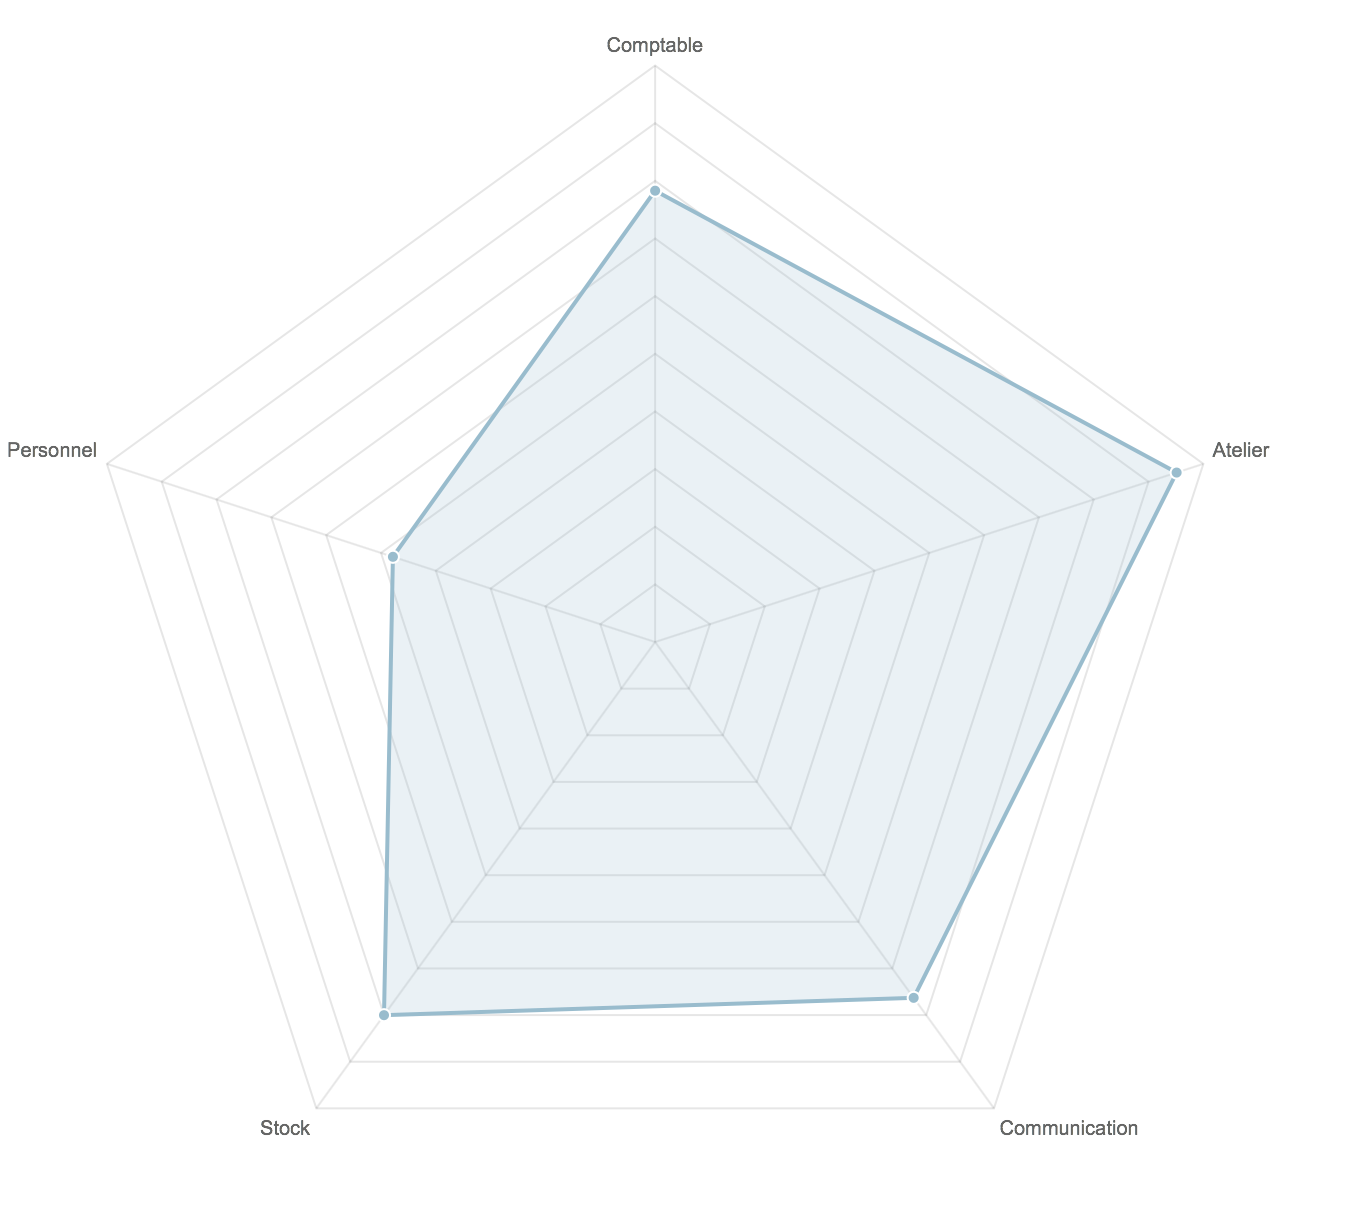
\includegraphics[scale=0.5]{../Partie2/Partie2.png}
        \caption{
            \label{fig} Niveau de satisfaction en fonction des objectifs de chaque responsable
        }
    \end{center}
\end{figure}
Nous trouvons cette solution satisfaisante car nous rognons seulement sur les objectifs du responsable personnel pour obtenir environ \textbf{80\% de satisfaction} concernant les objectifs des autres responsables. 
\newpage
\section{Analyse Multicritère}
\subsection{Choix de la méthode}
Nous recherchons la meilleure solution parmi les huit proposées\footnote{a,b,c,d,e,f,g,h ne font plus référence aux quantités de produits, ils feront désormais référence aux propositions de gestion} : pour cela, nous avons décidé d’utiliser la méthode Electre I, qui permet de trouver la meilleure solution. En parallèle, la méthode Electre II permet de classer les solutions, d’où le choix de la méthode Electre I.
\subsection{Mise en œuvre de la méthode}
\subsubsection{Solutions dominantes}
D’après la matrice d'appréciation, nous notons que les solutions suivantes dominent les autres solutions : a, b, d, e, h (Cf Figure 4).\\

\begin{figure}[H]
   \begin{center}
        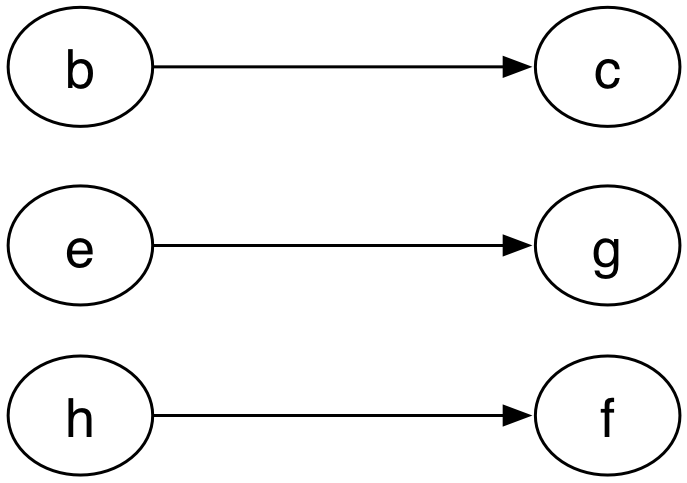
\includegraphics[scale=0.30]{../CR/src/Mimi/3eme.png}
        \caption{
           \label{fig} Rapports de domination directs
        }
    \end{center}
\end{figure}
L’étude s'effectuera en deux temps : dans un premier temps, nous allons considérer que tous les coefficients de pondération sont égaux à 1, puis, dans un second temps, les critères d’appréciation seront pondérés selon les résultats obtenus dans la partie 2.
\subsubsection{Analyse sans pondération}
Nous présenterons dans un premier temps la matrice \textbf{de concordance} :
\begin{center}
$ M_{Concordance} =\begin{pmatrix}
-&3/4&3/4&3/4&3/4\\
1/4&-&2/4&3/4&2/4\\
2/4&2/4&-&2/4&3/4\\
1/4&3/4&2/4&-&2/4\\
2/4&2/4&3/4&2/4&-\\
\end{pmatrix} $\\
\end{center}
Ensuite, la matrice \textbf{de discordance} que nous utiliserons dans l'analyse :
\begin{center}
$ M_{Discordance} =\begin{pmatrix}
-&4/10&2/10&4/10&2/10\\
2/10&-&3/10&6/10&1/10\\
3/10&4/10&-&5/10&2/10\\
2/10&6/10&3/10&-&4/10\\
3/10&2/10&2/10&5/10&-\\
\end{pmatrix} $\\
\end{center}

\emph{Premier seuillage :}\\
Dans un premier temps, on choisit les valeurs suivantes : 
\begin{center}
\textbf{$s = 0,75 = 3/4$\\
$v= 0,2 = 2/10$}
\end{center}
En comparant les matrices de concordance et de discordance aux seuils s et v, on obtient le résultat ci-dessous :\\
\begin{figure}[H]
   \begin{center}
        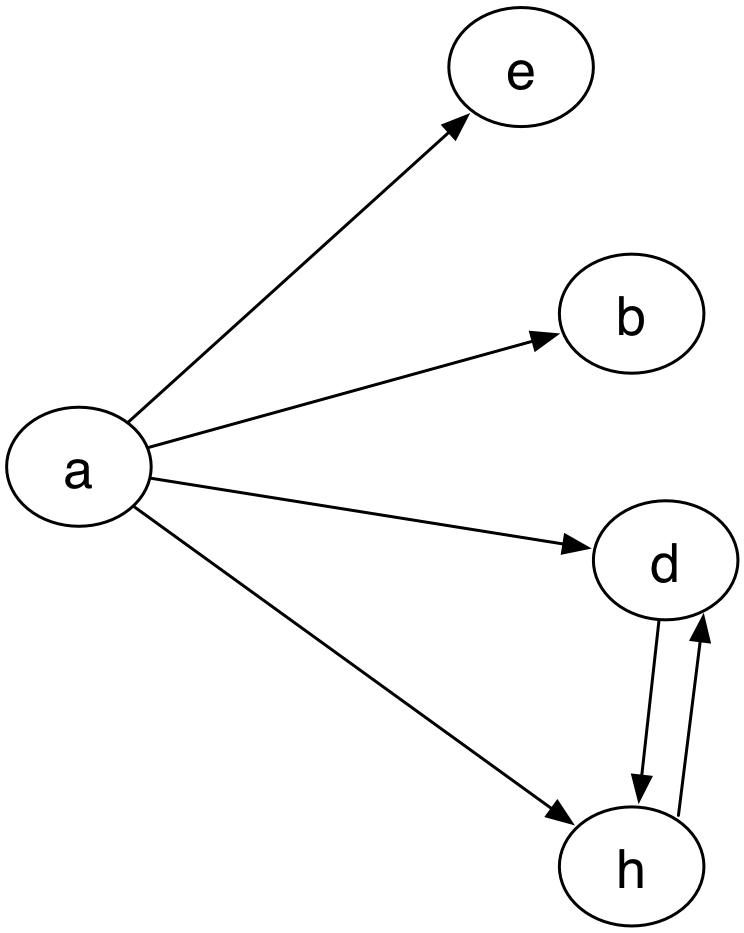
\includegraphics[scale=0.30]{../CR/src/Mimi/2eme.png}
        \caption{
           \label{fig} Resultats 1er Seuillage
        }
    \end{center}
\end{figure}
L’ensemble [a,b,e] constitue le noyau. Cependant, nous souhaitons obtenir une meilleure solution : le résultat obtenu n’est donc \textbf{pas satisfaisant}.\\\\

\emph{Deuxième seuillage :}\\
Afin d’affiner le résultat et de n’obtenir qu’une seule meilleure solution, on modifie les valeurs du seuil de discordance :\\
\begin{center}
\textbf{$s = 0,75 = 3/4$\\
$v= 0,4 = 4/10$}
\end{center}
En procédant de la même façon que pour le premier seuillage, on obtient le résultat suivant :\\
\begin{figure}[H]
   \begin{center}
        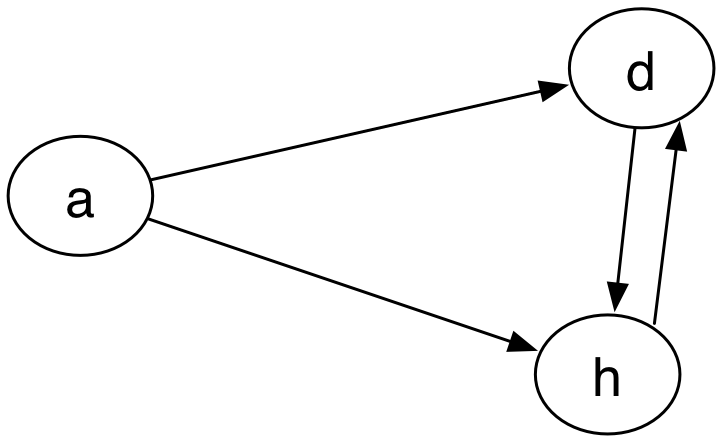
\includegraphics[scale=0.30]{../CR/src/Mimi/1er.png}
        \caption{
           \label{fig} Resultats 2eme Seuillage
        }
    \end{center}
\end{figure}
L’ensemble [a] constitue le noyau : \textbf{a est donc la meilleure solution} à ce problème.\\
\subsubsection{Analyse avec pondération}
Dans cette section, nous évaluerons l'impact de la solution optimale obtenue grâce à l'analyse multicritère sur l'appréciation des solutions proposées.\\
Ainsi, en se référant aux résultats de la deuxième partie, nous imposerons \textbf{un poids fort (4)} aux 3 critères suivants : \textbf{g1, g2 et g3} et \textbf{un poids faible (1)} au critère restant : \textbf{g4}. Nous changerons l'échelle de ce dernier critère à [3-7] afin de l'adapter au poids faible sus-mentionné.\\
La nouvelle matrice des jugements est la suivante :\\
\begin{table}[H]
\centering
\begin{tabular}{|l|l|c|r|r|}
  \hline
  Solutions & g1(4) & g2(4) & g3(4) & g4(1)\\
  \hline
  a &6 & 5 & 5 & 5 \\
  b &5 & 4 & 9 & 4.2 \\
  c &3 & 4 & 7 & 4.2 \\
  d &3 & 7 & 5 & 4.6 \\
  e &5 & 4 & 3 & 6.6\\
  f &2 & 5 & 7 & 4.2 \\
  g &5 & 4 & 2 & 6.6\\
  h &3 & 5 & 7 & 4.6\\
  \hline
\end{tabular}
\end{table}
De ce fait, les matrices \textbf{de concordance} et \textbf{de discordance} associées\footnote{a,b,d,e,h sont maintenues en position dominante} sont :
\begin{center}
$ M_{Concordance} =\begin{pmatrix}
-&9/13&9/13&12/13&9/13\\
4/13&-&8/13&12/13&8/13\\
8/13&5/13&-&8/13&9/13\\
1/13&9/13&5/13&-&5/13\\
8/13&5/13&9/13&8/13&-\\
\end{pmatrix}$
\end{center}
\begin{center}
$M_{Discordance} =\begin{pmatrix}
-&4/10&2/10&1.6/10&2/10\\
1/10&-&3/10&2.4/10&1/10\\
3/10&4/10&-&2/10&2/10\\
2/10&6/10&3/10&-&4/10\\
3/10&2/10&2/10&2/10&-\\
\end{pmatrix} $\\
\end{center}
\emph{Premier seuillage :}\\
Dans un premier temps, on choisit les valeurs suivantes : 
\begin{center}
\textbf{$s = 0,9 = 11.7/13$\\
$v= 0,1 = 1/10$}
\end{center}
En comparant les matrices de concordance et de discordance aux seuils s et v, on obtient le résultat ci-dessous :\\
\begin{figure}[H]
   \begin{center}
        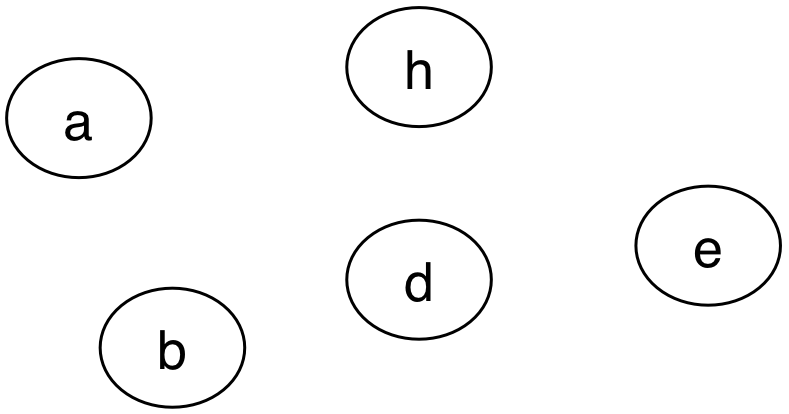
\includegraphics[scale=0.30]{../CR/src/Amine/1er.png}
        \caption{
           \label{fig} Resultats 1er Seuillage : Absence de solutions satisfaisantes
        }
    \end{center}
\end{figure}
L’ensemble {a,b,d,e,h} constitue le noyau. Ce seuillage est trop grossier et \textbf{non satisfaisant}.\\\\

\emph{Deuxième seuillage :}\\
Nous modifions les valeurs du seuil de discordance et revoyons les valeurs du seuil de concordance à la baisse :\\
\begin{center}
\textbf{$s = 0,69 = 8.9/13$\\
$v= 0,2 = 2/10$}
\end{center}
En procédant de la même façon que pour le premier seuillage, on obtient le résultat suivant :\\
\begin{figure}[H]
   \begin{center}
        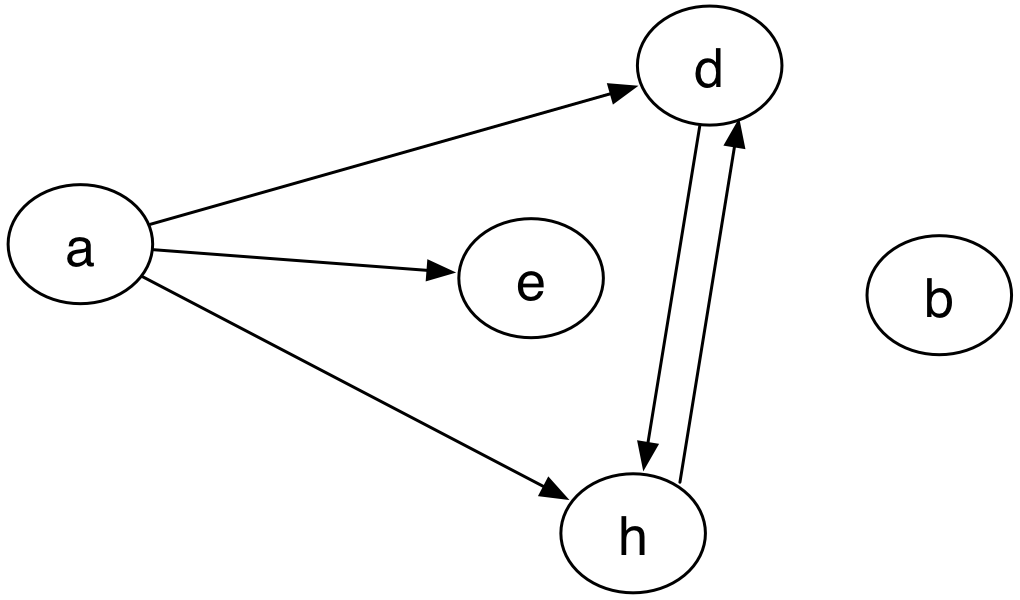
\includegraphics[scale=0.25]{../CR/src/Amine/3eme.png}
        \caption{
           \label{fig} Resultats 2eme Seuillage 
        }
    \end{center}
\end{figure}
L’ensemble {a,b} constitue le noyau, nous procèderons à un dernier seuillage pour dégager la meilleure solution.\\\\

\emph{Troisième seuillage :}\\
Nous modifions les valeurs du seuil de discordance :\\
\begin{center}
\textbf{$s = 0,69 = 8.9/13$\\
$v= 0,4 = 4/10$}
\end{center}
En procédant de la même façon que pour le deuxième seuillage, on obtient le résultat suivant :\\
\begin{figure}[H]
   \begin{center}
        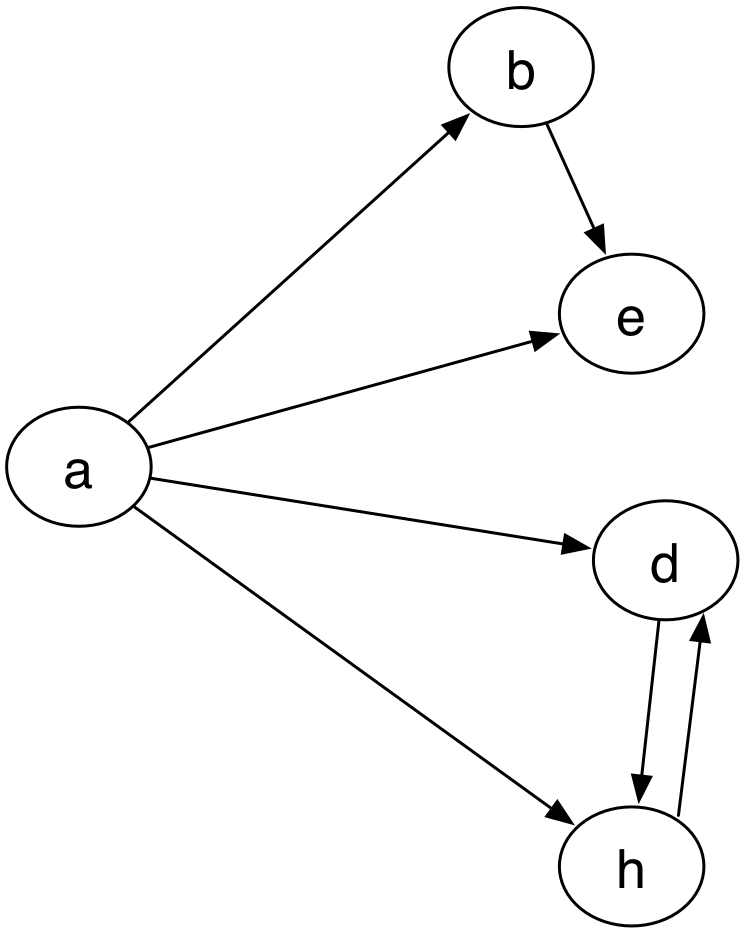
\includegraphics[scale=0.25]{../CR/src/Amine/4eme.png}
        \caption{
           \label{fig} Resultats 3eme Seuillage 
        }
    \end{center}
\end{figure}
L’ensemble {a} constitue le noyau : \textbf{a est donc la meilleure solution} à ce problème.\\
\newpage
\section*{Annexe}
\begin{lstlisting}
% Matrice de contraintes
A=[
    1 2 1 5 0 2;
    2 2 1 2 2 1;
    1 0 3 2 2 0;
    8 15 0 5 0 10;
    7 1 2 15 7 12;
    8 1 11 0 10 25;
    2 10 5 4 13 7;
    5 0 0 7 10 25;
    5 3 5 8 0 7;
    5 5 3 12 8 0
];
B = [350; 620; 485; 4800; 4800; 4800; 4800; 4800; 4800; 4800];  

%-------------------------------------------------------------------------------------------
function [ x ] = comptable( A, B )
%Cette fonction permet de calculer le benefice maximal pour le comptable
%et de calculer le nombre de chaque produits correspondant.

%Equation 
%5.67A + 11.88B + 12.27C + 1.03D + 31.65E + 27.55F

f = [-5.67; -11.88; -12.27; -1.03; -31.65; -27.55];
lb = [0;0;0;0;0;0];
x = linprog(f, A, B,[],[],lb); 

result = -f' * x
end

%-------------------------------------------------------------------------------------------
function [x] = respAtelier( A,B )
%Cette fonction permet de calculer le nombre de produit maximal a fabriquer

%Equation
%f(a,b,c,d,e,f) = a+b+c+d+e+f (maximiser)

f = [-1; -1; -1; -1; -1; -1];
lb = [0;0;0;0;0;0];
x = linprog(f, A, B,[],[],lb,[]); 

Result = -f'*x
end

%-------------------------------------------------------------------------------------------
function [ x ] = stock( )
% cette fonction permet de minimiser le stock global en integrant des
% contraintes supplementaires de production

A=[
    1 2 1 5 0 2;
    2 2 1 2 2 1;
    1 0 3 2 2 0;
    8 15 0 5 0 10;
    7 1 2 15 7 12;
    8 1 11 0 10 25;
    2 10 5 4 13 7;
    5 0 0 7 10 27;
    5 3 5 8 0 7;
    5 5 3 12 8 0;
    1 1 1 1 1 1;
    -1 -1 -1 -1 -1 -1; %(-) Car superieur ou egal 
];

R = zeros(100); %Resultat du stock
for i=1:100  
    B = [350; 620; 485; 4800; 4800; 4800; 4800; 4800; 4800; 4800; 378.8; -(i/100)*378.8];
    f = [5; 5; 6; 10; 5; 4];
    lb = [0;0;0;0;0;0];
    x = linprog(f, A, B,[],[],lb,[]);
    R(i) = f'*x;    
end

hold on
plot(R)
hold off;

    B = [350; 620; 485; 4800; 4800; 4800; 4800; 4800; 4800; 4800; 378.8; -(80/100)*378.8];
    f = [5; 5; 6; 10; 5; 4];
    lb = [0;0;0;0;0;0];
    x = linprog(f, A, B,[],[],lb,[]);
    f'*x
end

%-------------------------------------------------------------------------------------------
function [ x ] = COM( A, B, Aeq, Beq)
%Cette fonction permet de calculer et minimiser l'ecart de production
%entre les deux categorie de produit. Elle calcule le nombre de chaque 
%produits a fabriquer correspondant.

f=[-1 ; -1; -1; -1; -1; -1 ];
lb = [0; 0; 0; 0; 0; 0];
x=linprog(f, A, B, Aeq, Beq, lb, []);

end

%-------------------------------------------------------------------------------------------
function [ X ] = Pers()
%Cette fonction permet de calculer et minimiser le temps d'utilisation des
%machines 3 et 5, en integrant des contraintes supplementaires

A=[
    1 2 1 5 0 2;
    2 2 1 2 2 1;
    1 0 3 2 2 0;
    8 15 0 5 0 10;
    7 1 2 15 7 12;
    8 1 11 0 10 25;
    2 10 5 4 13 7;
    5 0 0 7 10 25;
    5 3 5 8 0 7;
    5 5 3 12 8 0;
    1 1 1 1 1 1;
    -1 -1 -1 -1 -1 -1; %(-) Car superieur ou egal 
];

R = zeros(100); %Temps machine total
R3 = zeros(100);%Temps machine 3
R5 = zeros(100);%Temps machine 5
for i=1:100
    
    B = [350; 620; 485; 4800; 4800; 4800; 4800; 4800; 4800; 4800; 378.8; -(i/100)*378.8];
    lb = [0;0;0;0;0;0;];

    f=[13;1;11;7;20;50];%fonction Temps machine total
    x = linprog(f, A, B,[],[],lb,[]);
    R(i) = f'*x;
    
    f=[8;1;11;0;10;25];%fonctionTemps machine 3
    R3(i) = f'*x;
    
    f=[5;0;0;7;10;25];%fonction Temps machine 5
    R5(i) = f'*x;
    
end

subplot(3,1,1), plot(R)
subplot(3,1,2), plot(R3)
subplot(3,1,3), plot(R5)


%solution optimale a 82%
    B = [350; 620; 485; 4800; 4800; 4800; 4800; 4800; 4800; 4800; 378.8; -(82/100)*378.8];
    lb = [0;0;0;0;0;0;];

    f=[13;1;11;7;20;50];
    x = linprog(f, A, B,[],[],lb,[]);
    f'*x
    
    f=[8;1;11;0;10;25];
    f'*x
    
    f=[5;0;0;7;10;25];
    f'*x
    
    x
end
%-------------------------------------------------------------------------------------------
%--------------------------------------Partie2---------------------------------------------

function [ Satisfaction ] = Satisfaction( Gain, Solt )
%Calcul de la matrice de satisfaction
%Elle nous donne la satisfaction de la solution par rapport au point de
%mire
%(Satisfaction entre 0 et 1)

Satisfaction = zeros(5,5);
Satisfaction(:,1) = Gain(:,1)./Gain(1,1);
%On veut un benefice maximal donc on divise le benefice par rapport a l'objectif ideal.

Satisfaction(:,2) = Gain(:,2)./Gain(2,2); 
%On veut un nombre de produit maximal donc on divise donc le nombre de produits par rapport a l'objectif ideal.

Satisfaction(:,3) = Gain(3,3)./Gain(:,3);
%On veut un stock minimal donc on divise donc l'objectif ideal par rapport au stock.

%Pour l'equilibre, nous regardons le rapport entre les deux familles pour
%obtenir la satisfaction. La satisfaction maximale est obtenue quand on
%peut a l'equilibre parfait.
for i=1:5;
    sol1 = (Solt(1,i) + Solt(2,i) + Solt(3,i)) / (Solt(4,i) + Solt(5,i) + Solt(6,i));
    sol2 = (Solt(4,i) + Solt(5,i) + Solt(6,i)) / (Solt(1,i) + Solt(2,i) + Solt(3,i));
    if sol1<1
        Satisfaction(i,4) = sol1;
    else
        Satisfaction(i,4) = sol2;
    end
end

Satisfaction(:,5) = Gain(5,5)./Gain(:,5);
%On veut un temps d'utilisation des machines minimal donc on divise donc l'objectif ideal par rapport au temps d'utilisation des machines.

end

%-------------------------------------------------------------------------------------------
function [ Satisfaction ] = VecteurSatisfaction( pointActuel, PM, sol )
%Calcul du vecteur de satisfaction
%Elle nous donne la satisfaction de la solution par rapport au point de
%mire

Satisfaction = zeros(5,1);
Satisfaction(1) = pointActuel(1)./PM(1);
%On veut un benefice maximal donc on divise le benefice par rapport a l'objectif ideal.


Satisfaction(2) = pointActuel(2)./PM(2);
%On veut un nombre de produit maximal donc on divise donc le nombre de produits par rapport a l'objectif ideal.


Satisfaction(3) = PM(3)./pointActuel(3);
%On veut un stock minimal donc on divise donc l'objectif ideal par rapport au stock.


%Pour l'equilibre, nous regardons le rapport entre les deux familles pour
%obtenir la satisfaction. La satisfaction maximale est obtenue quand on
%peut a l'equilibre parfait.
    sol1 = (sol(1) + sol(2) + sol(3)) / (sol(4) + sol(5) + sol(6)) ;
    sol2 = (sol(4) + sol(5) + sol(6)) / (sol(1) + sol(2) + sol(3)) ;
    if sol1<1
        Satisfaction(4) = sol1;
    else
        Satisfaction(4) = sol2;
    end
    
    
Satisfaction(5) = PM(5)./pointActuel(5);
%On veut un temps d'utilisation des machines minimal donc on divise donc l'objectif ideal par rapport au temps d'utilisation des machines.

end

%-------------------------------------------------------------------------------------------
function [] = Partie2()
%---Solutions Partie 1 ---%
F_compta = [-5.67; -11.88; -12.27; -1.03; -31.65; -27.55];
F_respAtelier = [-1; -1; -1; -1; -1; -1];
F_respStock = [-5; -5; -6; -10; -5; -4];
F_respCom=[-1;-1;-1;1;1;1];
F_respPers=[-13;-1;-11;-7;-20;-50];

sol_compta = [0;20.41;0;0;242.5;94.18];
sol_respAtelier = [0;56.73;38.69;0;184.46;98.92];
sol_respStock = [38.3473;25.4708;0.0000;0.0000;108.8663;130.3556];
sol_respCom = [142.12;0;44.42;0;104.81;81.73];
sol_respPers =[0;174.38;1.23;0;135;0];
%---Fin Solutions Partie 1 ---%


%---Calcul Matrice Gain---%
Ft = [F_compta,F_respAtelier,F_respStock,F_respCom,F_respPers];
Solt = [sol_compta,sol_respAtelier,sol_respStock,sol_respCom,sol_respPers];

PM = [10512; 378.8; 1385; 0; 2887.9];  %Point de Mire

Gain = -transpose(Solt)*Ft
%---Fin Calcul Matrice Gain---%

Satisfaction(Gain, Solt) %Matrice de Satisfaction

%---Ajustement de la solution ---%
%On place Tous les responsables sauf le compta en contrainte, 
%on ajuste puis on recalcule
A=[
    1 2 1 5 0 2;
    2 2 1 2 2 1;
    1 0 3 2 2 0;
    8 15 0 5 0 10;
    7 1 2 15 7 12;
    8 1 11 0 10 25;
    2 10 5 4 13 7;
    5 0 0 7 10 25;
    5 3 5 8 0 7;
    5 5 3 12 8 0;
    -1 -1 -1 -1 -1 -1; %Resp Atelier
    -5 -5 -6 -10 -5 -4; %resp Stock
    -1 -1 -1 1 1 1; %resp Comm
    -13 -1 -11 -7 -20 -50; %resp Perso
];


%Reduire produits 378.8
%Augmenter Stock 1385
%Reduire ou augmenter Comm
%Augmenter Personnel 2887.9
B = [350; 620; 485; 4800; 4800; 4800; 4800; 4800; 4800; 4800; -358.8; -1385; -0; -2887.9];
B = [350; 620; 485; 4800; 4800; 4800; 4800; 4800; 4800; 4800; -320; -1425; 25; -3075];
B = [350; 620; 485; 4800; 4800; 4800; 4800; 4800; 4800; 4800; -340; -1450; -25; -2990];
B = [350; 620; 485; 4800; 4800; 4800; 4800; 4800; 4800; 4800; -290; -1490; -25; -3090];
B = [350; 620; 485; 4800; 4800; 4800; 4800; 4800; 4800; 4800; -339; -1425; 70; -2575];
B = [350; 620; 485; 4800; 4800; 4800; 4800; 4800; 4800; 4800; -339; -1425; 40; -3075]; %Solution Retenue


sol_comptable = comptable(A,B);

PM = [10512; 378.8; 1385; 0; 2887.9]; %Point de Mire  
pointActuel = [-F_compta' * sol_comptable; -F_respAtelier' * sol_comptable; -F_respStock' * sol_comptable; -F_respCom' * sol_comptable; -F_respPers' * sol_comptable]

VecteurSatisfaction(pointActuel, PM, sol_comptable)

end
\end{lstlisting}
\end{document}